\documentclass[a4paper]{danarticle}
\usepackage{a4}
\usepackage[dvips]{color}
\usepackage[dvips]{graphicx}
\usepackage{amsthm}
\pagestyle{headings}
\sloppy
 
 
\begin{document}
  \author{Daniel Hahn}
  \title{Finding Visitor-Related URLs (Draft)}
  \maketitle
  
  \section*{Introduction}
    This article explains an system for finding URLs wich are
    \textit{related} to a specific \textit{visit}. To understand the
    function of the system it is neccessary understand
    some of the underlying terms and concepts.
    
    \textbf{A visit} in a real-life-system is (in most cases) the
    act of a person (or machine) requesting some document from a
    web server. However, it is easy to imagine that the system will
    also deal with other types of visits (like signing up to a
    chat system or even physically coming to a place). For this
    reason\footnote{And also to convey a more intuitive understanding
    of the system.} we will generally use generic phrases (like \lq 
    virtual place\rq ) instead of web-specific technical terms (such
    as \lq web page\rq ). Finally, for the algorithms used in the
    system a \textbf{visit} is nothing more than a collection of
    data, which in our example corresponds with a line in the web
    server's log file. Whenever we want to distinguish between the
    actual event of a visit taking place and the set of data
    describing this event we will call the former a \textit{visit event}
    
    \textbf{Relations between visits and URLs.} A simple example
    for a relationship between a visit and an URL could be
    \lq\lq The URL is in the same domain the visit came from\rq\rq .
    However, it is important to note that the nature of those 
    relations has to be specified by the user: The system will 
    \textit{not} find any \lq new\rq\ relationsships, nor has it 
    any idea of what those relations actually \lq mean\rq .\footnote{This
    is fuzzy enough to warrant a little example: While you may tell the
    system something like \lq Look at this visit and find me web 
    pages that are in the same domain as the visitor\rq\ you cannot
    simply make requests like \lq Find out what this visitor was 
    interested in and give me a list of people who share this
    interest\rq .} 
    
  \section*{System overview}
    \begin{figure}
      \centering
      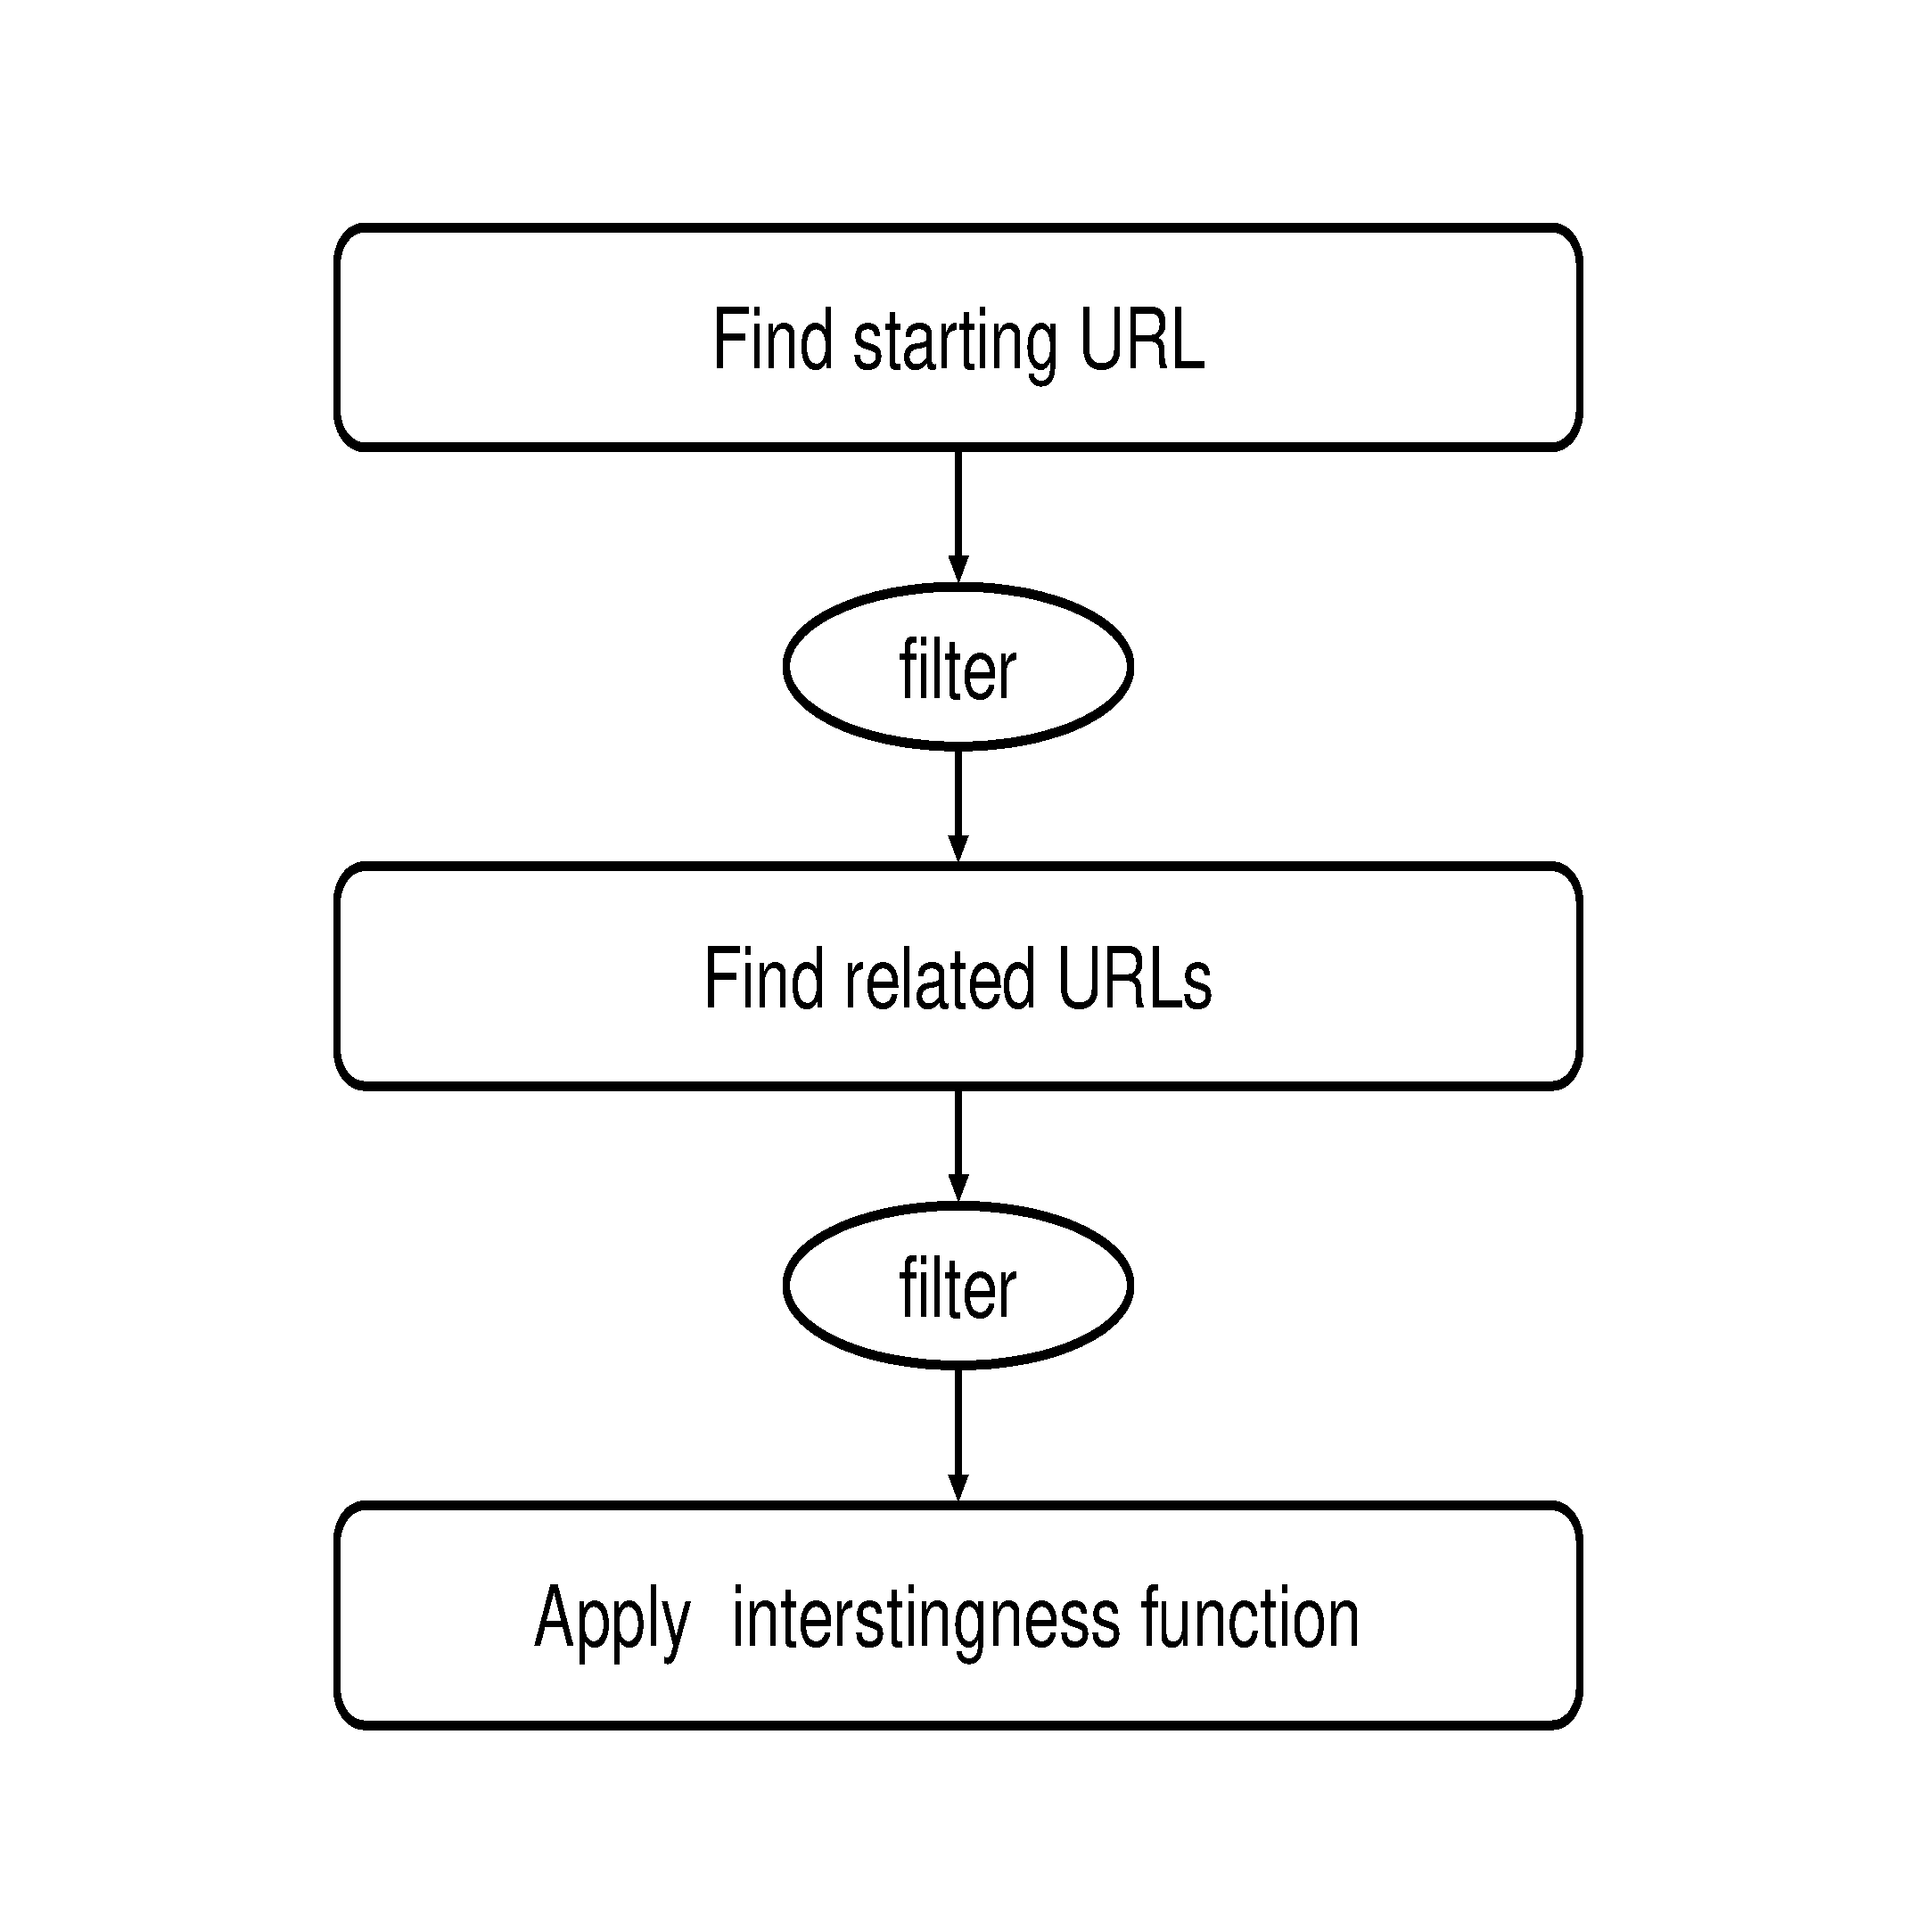
\includegraphics[width=10cm]{steps_overview.eps}
      \caption{System Overview}
    \end{figure}
  \section*{Step one: Find the starting point}
    Our system attempts to find URLs which are \textit{related} to
    a given visit. However, it is much more difficult to describe
    a relationship between a visit and an URL than the relationship
    between two URLs.
    
    For this reason we want to \textbf{use a single URL as the
    starting point} for our search. Additionally we demand that
    \textbf{this URL is as \textit{close as possible} to the
    origin of the visit.}\footnote{This does not neccessarily
    mean that the URL is close to the \textit{visitor}, because
    the visit may contain no information about the \textit{visitor}
    at all.}
    
    \subsection*{How is an URL close to the origin of a visit?}
      It is safe to assume that there can be different meanings
      of \textit{close} for differnt types of visits. Still, when
      dealing with a visit that was originally an http request,
      the meaning of \textit{close} is reasonably easy to define:
      
      The \textit{origin} of such a visit is the IP address or
      hostname\footnote{For the sake of convenience we will simply
      assume that whenever possible an IP addess will be translated
      into a valid DNS hostname.}. The \textbf{closest possible URL}
      would therefore be the URL describing this address, but it
      may have the drawback of not being \textit{alive}\footnote{We
      will call an URL \textit{alive} when there is a HTTP server
      answering GET or HEAD requests for this URL.}.
      
      For applications where it is desireable to have a starting
      URL that is \textit{alive}, we will therefore try to find the
      URL \textit{closest} to the \lq startin\rq\ URL describing
      the the \textbf{origin} and is still alive. For this, we 
      will use the follwowing definition of \textit{close}:
      An URL is \textit{closer} to one in the same subdomain 
      than to one in a different subdomain. (E.g.: \textit{i.am.here.com}
      would be closer to \textit{visitor.am.here.com} than
      \textit{elswhere.here.com}, but this would still be closer than
      \textit{somewhere.else.org}). If the original URL describes only
      an IP address we say that an URL is \textit{closer} to one
      in the same subnet than to one on a different network.
  \section*{Step Two: Finding Related URLs}
     \begin{figure}
       \centering
       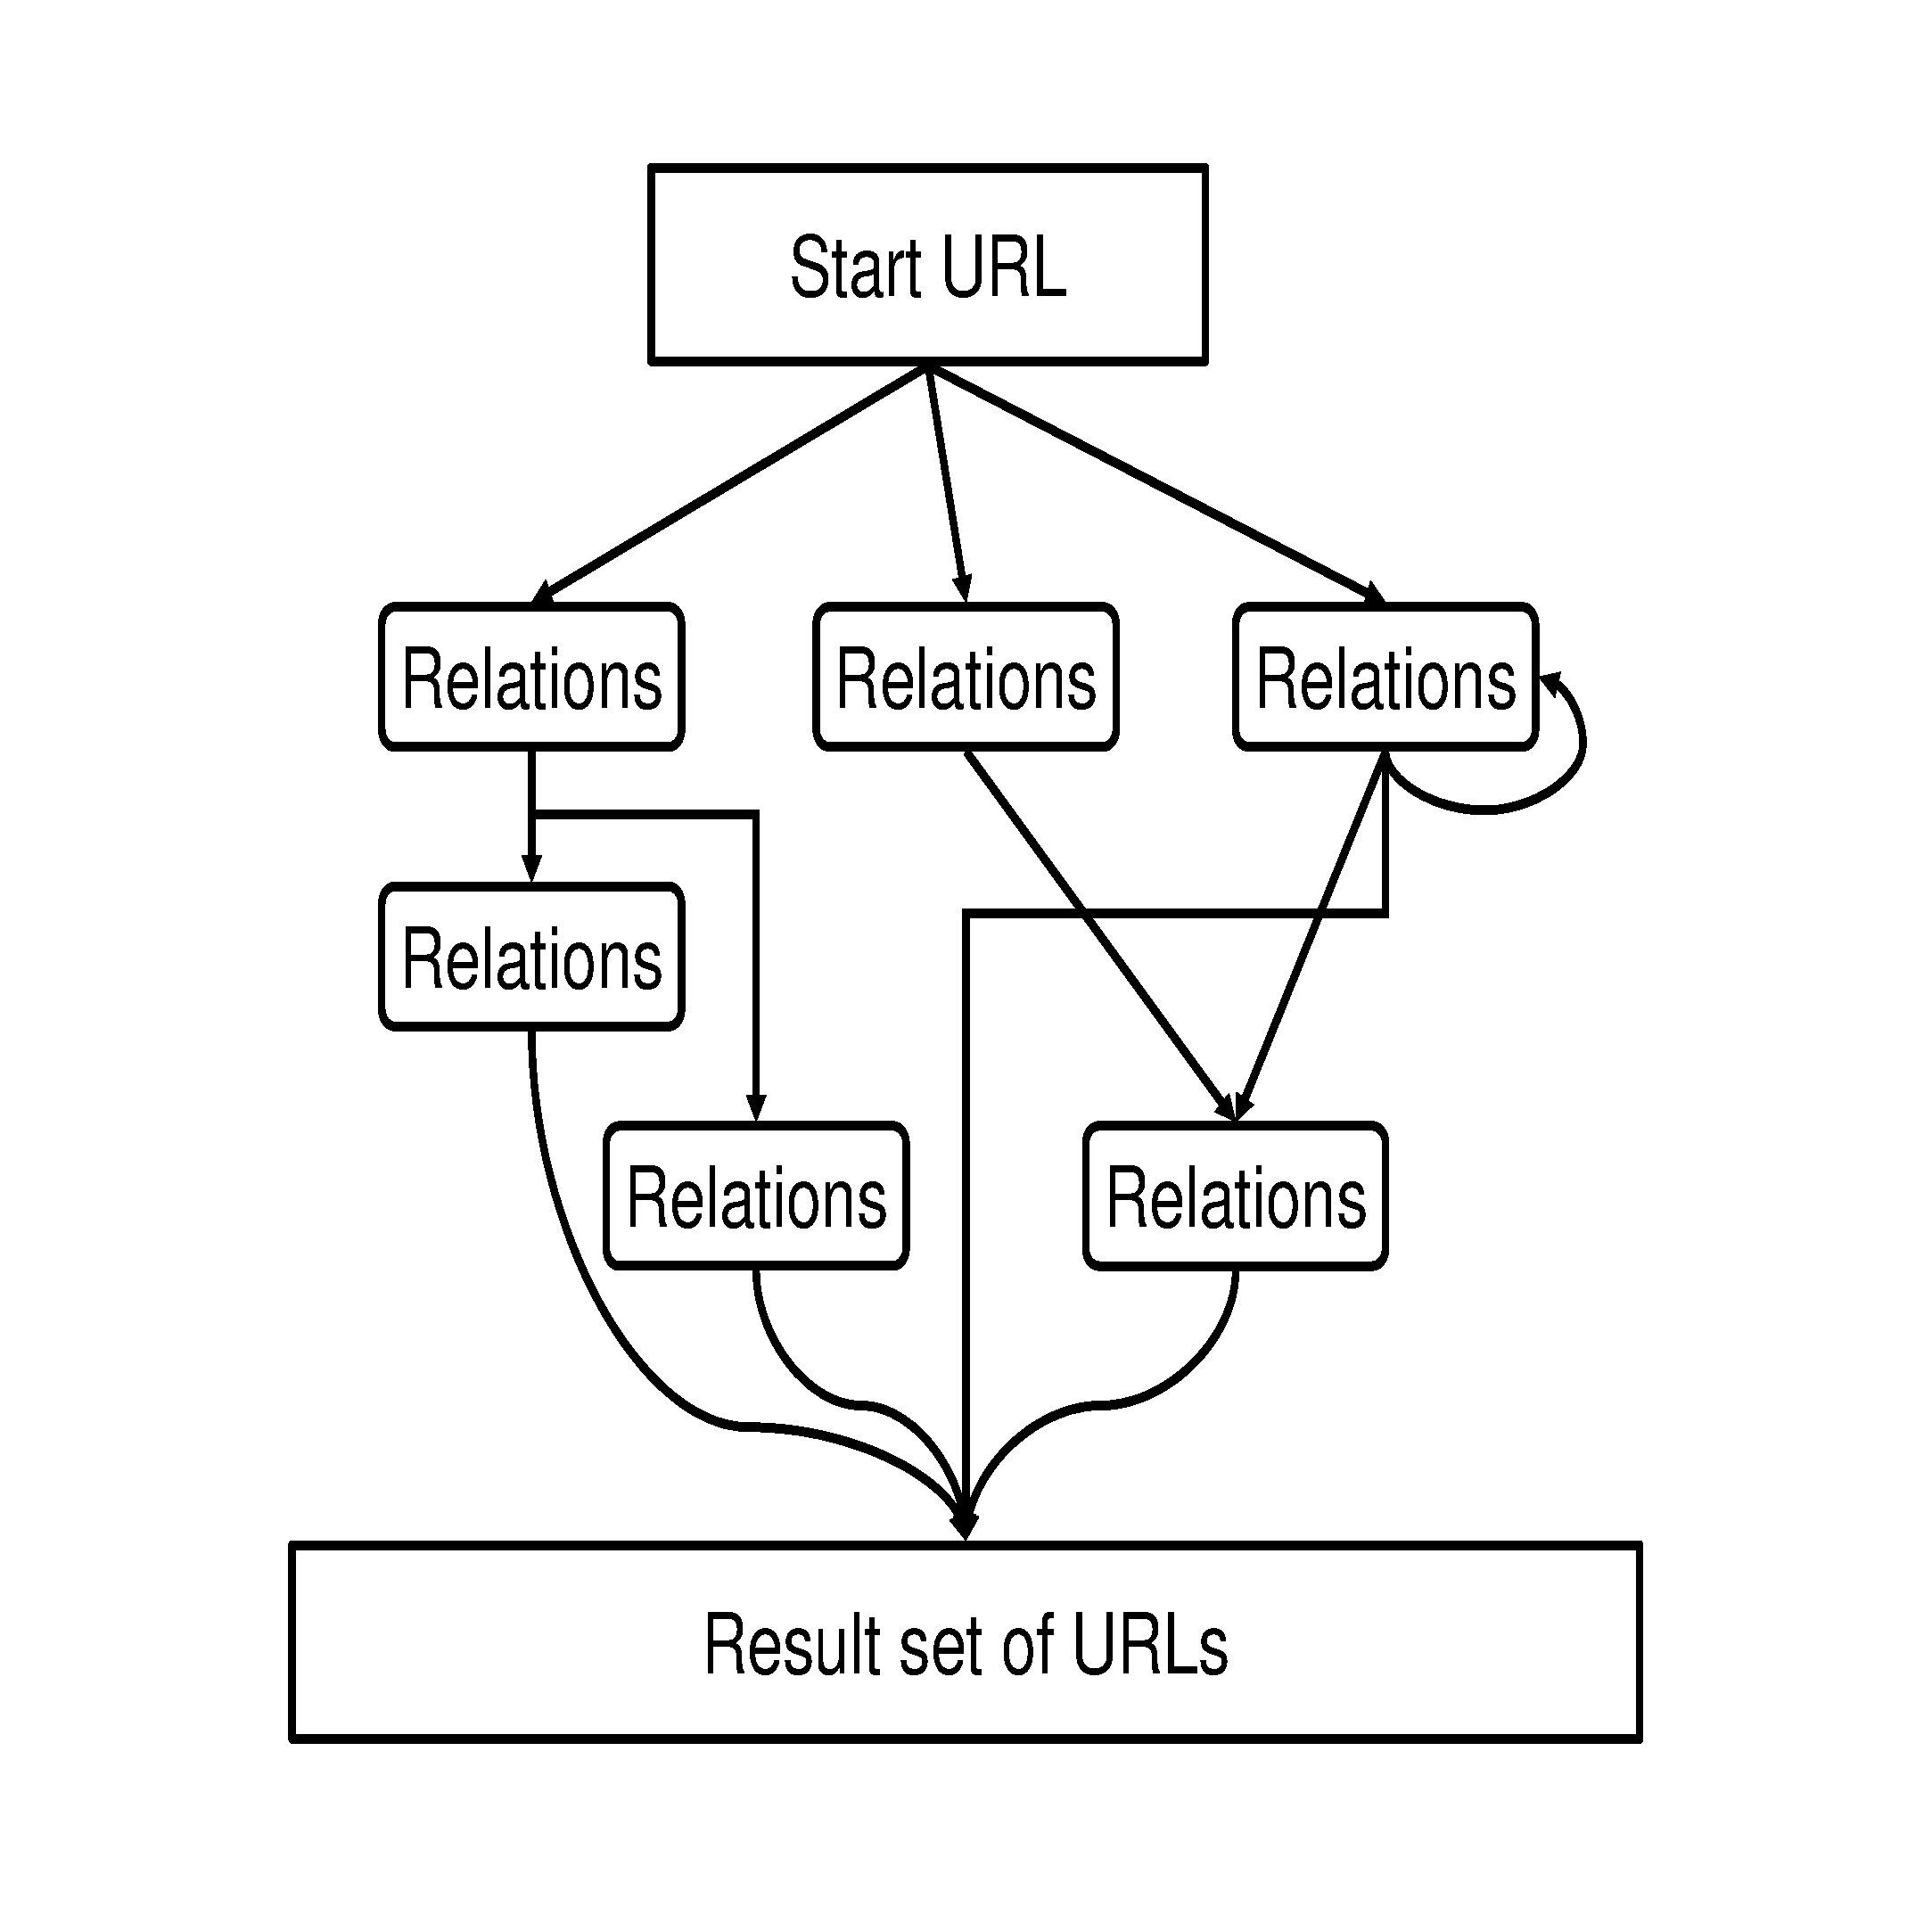
\includegraphics[width=10cm]{relations.eps}
       \caption{Data flow through multiple relation-finding instances}
     \end{figure}
     This is the meat and bones of the system: Starting with the
     URL we found in the first step we will start to search for
     URL that \textbf{are related to the starting URL}
     and we will say that
     \textbf{two URLs are related when they share a common
     characteristic}. 
     
     The system has no preconception about such characteristics other
     than that -- for a real-world system -- pages with that 
     characteristic must be resonably easy to 
     find.\footnote{Which is somehow
     obvious: While it makes perfect sense to say that URLs can
     be related by the fact that the web author's grandmothers share
     the same maiden name one will be hard-pressed to find an
     algorithm that looks for such URLs} The system may also
     look for different kinds of relationships, simply by
     repeating this step.
     
     We do \textbf{not} demand that this steps finds \textit{all}
     related URLs (since this would be quite impossible).
     
     \subsection*{Examples for relations between URLs}
       \begin{itemize}
         \item{The URLs are in the same domain.}
         \item{The URLs are found by a web search using the same keywords.}
         \item{The URLs contain documents containg similiar keywords}
       \end{itemize}
     
     \subsection*{Different degrees of relationship}
       The result of this processing step is a set of URLs $ U_{1} $,
       which containg URLs directly related to the starting
       URL by some relationship $ \leftrightarrow $. 
       We call these URLs \textit{related in the
       first degree} to the starting URL.
       We may continue to look for URLs \textit{related in the second
       degree} by taking each URL $ u \in U_1 $ and finding URLs related
       to $ u $. The set $ U_2 $ of URLs related in the second degree would
       then be:
       \[
        U_2 = \bigcup_{u \in U_1} u_2 \leftrightarrow u
       \]
       (For pratical reasons we assume that each URL is always related
       to itself, and thus $ U_1 \subset U_2 $)
       
       The process can be repeated to find URLs related in the 
       $ 3^{rd} $ and $ 4^{th} $ degree, and so on.
     \subsection*{Multiple instances}
       The system may contain any number of instances searching
       for relations\footnote{An \textit{instance} in this
       context is a program entity that takes a URL (or a
       set of URLs) and finds URLs that are related to it (them)
       by a given relation.}. There may be different instances
       for different relations, and there may also be multiple
       instances looking for the same relation. 
       
       The starting URL may be fed into any of those instances
       (which will the find URLs related in the $ 1^{st} $
       degree). 
       
       Each instance may pass it's output on to the next stage
       of processing, or feed it into one or more other instance(s) 
       (including itself), which will then find URLs with higher
       degrees of relationship. The system does not demand that
       instances that are \lq chained\rq in this way work with
       the same relations. 
       
       This kind of design allows for a very flexible configuration
       of this phase, making detailled decisions about the kind
       of relationships the system is looking for.
       Nonetheless, it may prove that overly complex configurations
       will not prove useful for real-world implementations.
     \subsection*{Note on finding relations in the real world}
       While in theory the nature of the relationships is only
       limited by the user's phantasy, a real-world implementation
       has to work on the available data\footnote{See Appendix for
       description of the available data}. Relations used in a
       real-world system should therefore match the following
       criteria:
       \begin{itemize}
         \item{Given the available data, it must be possible to
	       tell wether two URLs are related or not}
	 \item{It must be possible to find a set of 
	       URLs that \textit{may} be related with
	       a resonable effort.}
       \end{itemize}
       \textbf{It is important} to note that the URL is \textbf{not}
       the only input to the relation-finding process. Other information
       (e.g. the REFERER field for a specific visitor) may also be used.
  \section*{Step three: Finding URLs of interest}
    In the previous step were looking for a (probably rather large)
    set of URLs which are all somehow related to the original visit.
    Since we want to present these URLs to a user, it is now 
    neccessary to order them and find out which of them are most
    \textit{interesting} for the user. 
    The concept of \textit{intersting to the user} is again quite 
    hard to grasp algorithmically. We will therefore
    approximate \textit{interesting} with \textit{has certain
    properties that may make it interesting to the user} (e.g.
    the page contains certain keywords). Each of this properties
    shall be expressed by an \textit{interest function} $ f_i $ 
    that will assign a value $ 0 \leq i \leq 1 $ to a given URL
    $ u $. The system may use multiple \textit{interst functions}
    to check for different aspects that may be interesting
    to the user and assign a weight $ \alpha_{i} $ to each 
    of the functions. Thus, the overall \textit{interestingness}
    $ \iota $ of a URL would calculate to:
    \[
      \iota(u) = \sum_i \alpha_i f_i(u)
    \]
  
  \section*{Filtering}
    The system will allow for filters to be applied before each
    processing step, and again after applying the 
    \textit{interest functions} (this is before displaying the
    results). A real-world-system will probably also filter 
    the \textit{visits}, electing to discard some visits before
    doing anything else.
    
    Filtering is mainly a way to remove unwanted \lq noise\rq\ and
    speed up processing, it does not change the working of the
    system in a significant way
  \newpage
  \section*{Appendix: Available Data}
  \subsection*{Primary data from the visits}
    This is the \textit{primary} data form the visit itself.
    \begin{itemize}
    	\item{The \textit{origin} of the visit. (e.g.
    	      client's net address)}
    	\item{The \textit{resource} that was requested. (The document
    	      the visitor tried to download)}
    	\item{The \textit{time and date} of the visit.}
    	\item{The \textit{result} of the visit. (Successful or not?)}
    	\item{The \textit{referring entity}. (e.g. from the http REFERER field)}
    	\item{The \textit{user agent} that was used for the visit.}
    \end{itemize}
   \subsection*{Secondary data}
    This is secondary data, which is not recorded with the visits
    but available through other means (in a web system).
    \\
    \textbf{Information available through the context of the visit:}
    This kind of information is not directly recorded with the visit,
    but is easily available when one has additional knowledge of the
    context. Some examples would include:
    \begin{itemize}
    	\item{The geographical location. (Can be roughly deduced if 
    	      one has an idea about country-top-level-domains)}
    	\item{The type of visitor (e.g. human/machine/attacker,
    	      can be known by looking at the user agents and
    	      at patterns in the requests)}
    	\item{Search queries contained in the REFERER.}
    \end{itemize}
    \textbf{Information available through the web:} This includes
    all kinds of web services (most notably: search engines) as
    well as the information gained by actually querying a given
    URL. The latter will yield information such as:
    \begin{itemize}
    	\item{The fact if there is a web server answering.}
    	\item{The type of document served by that machine.}
    	\item{The document itself.}
    	\item{In the document: Meta descriptions (e.g. keywords)
    	      and links to other pages.}
    \end{itemize}
    \textbf{Information available through the network:} This is
    provided by services of the underlying network. This can
    be things like network routes (traceroute), names and addresses
    (DNS) or administranational information (WHOIS).
    \\
    \textbf{Information from the visitor:} It is imaginable that
    a visitor provides additional information upon each visit. 
    This could be things like the visitor's homepage, the 
    bookmark collection or simply the history of accesses.
\end{document}
